documentclass[10pt,a4paper]{article}
\usepackage[latin1]{inputenc}
\usepackage{amsfonts}
\usepackage{amsmath}
\usepackage{amssymb}
\usepackage{color}
\usepackage{graphicx}
\usepackage{hyperref}
\usepackage{enumitem}
\usepackage{graphicx}
\usepackage{array}
\usepackage{float}
\usepackage{pdfpages}
\usepackage{tcolorbox}

\usepackage[raggedright]{titlesec}
\usepackage[tmargin=3cm,bmargin=2.5cm,lmargin=1.3cm,rmargin=1.5cm]{geometry}
\hypersetup{
	colorlinks=true,
	linkcolor=black,
	filecolor=magenta,
	urlcolor=cyan,
}
\usepackage{sectsty}

\sectionfont{\LARGE}
\subsectionfont{\Large}
\subsubsectionfont{\Large}
\paragraphfont{\large}


\setcounter{secnumdepth}{5}

\newcolumntype{C}[1]{%
	>{\vbox to 2.5ex\bgroup\vfill\centering\arraybackslash}%
	p{#1}%
	<{\vskip-\baselineskip\vfill\egroup}}  

\author{\vspace{0.4cm}
	\Large{Anirudh N J}\\\vspace{0.4cm}
	\Large{Somesh Devagekar} \\\vspace{0.8cm}
	\Large{Raina Thomas}}

\title{
	\vspace*{5cm}
	\textbf{\Large{Scientific Experimentation and Evaluation}}
	}
	
\date{May 08, 2019}			
\begin{document}

\begin{titlepage}

	\maketitle
	
\end{titlepage}

	\Large
	\tableofcontents
	\newpage



\section{Task 1 : Manual Motion Observation}

\subsection{Aim}
\Large
The aim of this project is to construct a LEGO NXT differential drive robot and measure the observable end pose variation for three different trajectories: an arc to the left, driving straight and an arc to the right.
\vspace{0.5cm}

The experiment of measuring the end pose was done by measuring the pose using aruco markers and Computer Vision.
   

\subsubsection{Experimental Setup}
	
	\subsubsection{Software Setup}
		\vspace{0.3cm}
	\textbf{Software Installation}\\
			
		The following softwares were installed in the PC for driving the robot :
			\vspace{0.3cm}
			\begin{enumerate}
				
				\item
				Java SE Development Kit 8 was installed in the Windows Operating System of the PC. The software was downloaded from the website :\\ \href{https://www.oracle.com/technetwork/java/javase/downloads/jdk8-downloads-2133151.html}{https://www.oracle.com}
				\vspace{0.2cm}
				
				\item
				Eclipse IDE for Java Developers was downloaded and installed from the website 
				\href{http://eclipse.bluemix.net/packages/neon/?JAVA-WIN32}{http://eclipse.bluemix.net}. This IDE is the platform used for developing the program for driving the robot.
				\vspace{0.2cm}
				
				\item
				The leJOS NXT Fantom Driver was downloaded from  \href{https://www.lego.com/en-us/mindstorms/downloads}{https://www.lego.com/en-us/mindstorms/download}. 
				\vspace{0.2cm}
				
				\item
				The leJOS NXJ software was downloaded from \href{https://sourceforge.net/projects/nxt.lejos.p/files/}{https://sourceforge.net} and installed in the PC using the Windows Installer.
				\vspace{0.2cm}
				
				\item
				The leJOS NXJ plug-in was added to Eclipse.
				\vspace{0.5cm}
								
			\end{enumerate}
			\vspace{0.3cm}
			\textbf{Programming the robot}
	
			\begin{enumerate}
				\item
				The Lego NXT Java template code provided in the website below was modified for use in the robot.
				\href{https://lea.hochschule-bonn-rhein-sieg.de/ilias.php?ref_id=571436&cmd=view&cmdClass=ilrepositorygui&cmdNode=t3&baseClass=ilrepositorygui}{https://lea.hochschule-bonn-rhein-sieg.de}
				\item
				A LeJOS NXT Project was created in Eclipse and the template code was added to the project and certain parameters in the code was modified. The parameters that were modified for our experimental setup are given in the table below.				
					
				\begin{table}[ht]				
					\centering
				\begin{tabular}{ | C{3cm} | C{3cm}|  C{7cm} |} 
					\hline
					\textbf{Parameter} & \textbf{Value} & \textbf{Reason}\\ 
					\hline
					SLEEP\_TIME   & 3000.0 &  Increased to make the robot drive for a longer duration\\ 
					\hline
					TURN\_RATE  & 10.0 & Decreased to prevent the robot from making sharp turns\\ 
					\hline
				\end{tabular}
					\caption{Modified Code Parameters}
				  	\label{Tab:Tcr}
				\end{table}
		\item
		The NXT Device was connected to the PC via a USB Cable. The NXJ firmware was flashed into the device. The modified code was compiled and run as an LeJOS NXT Program to create a .nxj file. This was automatically flashed into the NXT device that was connected to the PC.
				
				
			\end{enumerate}
			
			
	
	\subsubsection{Hardware Setup}	
To reproduce the experiment the following equipments are required :
\begin{enumerate}
    \item
    White A0 Grid Sheet
    \item
    Camera - Microsoft 
    \item
    Assembled robot - Lego NXT 
    \item
    Scales for measuring the length 
    \item
    Vision markers
\end{enumerate}
\vspace{0.5cm}

The general steps to setup the experiment are as following :
\begin{enumerate}
    \item
    Place the White A0 sheet on a flat surface.  Try to remove any bends in the sheet and keep the paper as flat as possible. This will be called the 'map' on which the robot will move on. The measurement system is made of the robot, scale, camera, aruco markers and a paper. 
    \item
    Draw the template drawing of the "floor space" taken by the robot as shown in the figure. Concept of 'Behavior-shaping constraint'\footnote{Behavior shaping constraint : It is a type of design constraint to prevent the user from using the system in a way that it is not intended to be used in. In the case of the template given, the triangle prevents the robot to be placed in the reverse direction.} is used to prevent wrong initial placement of the robot.
    
    
    \begin{figure}[H]
	\centering
    \includegraphics[width=0.6\linewidth ]{Apparatus/map_small.png}
    \caption{ Template of the map}
    \end{figure}    
      
    \begin{figure}[H]
    	\centering
    	\includegraphics[width=0.6\linewidth ]{Apparatus/camera_placement.png}
    	\caption{Top view of the experimental setup without camera}
    \end{figure}
    
    \begin{figure}[H]
    	\centering
    	\includegraphics[width=0.6\linewidth ]{Apparatus/experiment_apparatus_01_small.png}
    	\caption{Top view of the experimental setup}
    \end{figure}
    
    \begin{figure}[H]
     	\centering
     	\includegraphics[width=0.55\linewidth ]{Apparatus/apparatus_front_view.png}
     	\caption{Front view of the experimental setup}
    \end{figure}
    
	\item
	Four aruco markers of different ids are used to find the corners of the grid sheet. The aruco markers are aligned such that the first corner of the marker which is detected by the CV algorithm overlaps with the corner of the sheet.
	\item
	The markers are also aligned to be perfectly parallel to the sheet edges. These markers should be aligned properly since the next preprocessing steps are dependant on this.
	\item
	The camera is placed rigidly such that the whole sheet is visible and the centre of the camera points approximately to the centre of the sheet.	
    \item
    The robot was assembled using the manual given with the LEGO NXT box. The robot firmware was flashed as given in the Software Setup. 
    \item
    We assumed that the driving axle is towards the front(leading edge) of the robot and that the robot origin lies in the centre of the driving axle.
    \item
    The two aruco markers on the robot are placed as ahown in the figure in such a way that one of the markers lies directly on top of the origin of the robot.
    \item
    Place the robot on the A0 sheet over the marked template in such a way that the castor wheel is turned outwards from the robot.
    \item
	The measurands are the coordinates of the robot's markers on the camera.
    
\end{enumerate}
\vspace{0.5cm}

The reference images of the DUT and the proposed marker tracking visualization are given below.

\begin{figure}[h]
	\centering
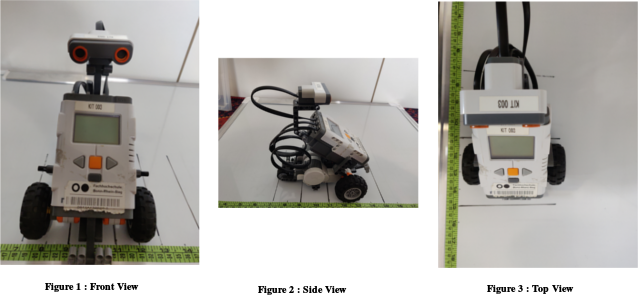
\includegraphics[width=0.9\linewidth ]{Apparatus/pose.jpeg}
\caption{ Views of the DUT}
\end{figure}

\subsubsection{Camera Calibration}


Calibration in computer vision is the method to find the intrinsic and extrinsic parameters of a particular camera. The intrinsic parameters of a camera deals with the physical qualities of the camera like focal length , skew , distorsion etc. Whereas, the extrinsic parameters of the camera deals with finding the pose of the external world with respect to the camera.\\

The general methods to perform the calibration are as follows.

\begin{enumerate}
	\item
	Download the image of the checkerboard pattern from the link given below.
	\href{https://boofcv.org/images/2/23/Calibration_letter_chessboard_7x5.png}{https://boofcv.org/images/2/23/Calibration\_letter\_chessboard\_7x5.png}
	
	\item
	Take a printout of the pattern on an A4 sheet and mount it on a rigid surface. This will be called as the target.
	
	\item
	Use the camera to be used in the setup to take pictures of the target at different orientation and distances.
	
	\item
	Use the OpenCV code given in the below link to get the calibration parameters for the camera. 
	\href{https://docs.opencv.org/3.4.3/dc/dbb/tutorial_py_calibration.html}{https://docs.opencv.org/3.4.3/dc/dbb/tutorial\_py\_calibration.html}
	
	\item
	The calibration parameters that are found will be used for removing the errors like barrel, radial distorsion and also to find the precise 3D pose of the marker in the image.


\end{enumerate}

\subsection{General Terms Formalization}


	\begin{itemize}
		\item	
		\textbf{Measurand :}
		\begin{itemize}
			\item
			Pose (x-coordinate, y-coordinate, orientation)
		\end{itemize}
		
		\item
		\textbf{Measurement :}
		\begin{itemize}
			\item
			Distance (mm)
			\item
			Angle (degrees)
		\end{itemize}
		\item
		\textbf{Measuring Principle :}
		\begin{itemize}
			\item
			Computer Vision
		\end{itemize} 
		\item
		\textbf{Measurement facility :}
		\begin{itemize}
			\item
			Camera
		\end{itemize} 
		\item
		\textbf{Device Under Test (DUT):}
		\begin{itemize}
			\item
			Lego NXT
		\end{itemize} 
		\item
		\textbf{Measurement System :}
		\begin{itemize}
			\item
			Grid Sheet
			\item
			Markers
			\item
			Camera
		\end{itemize}
		\item
		\textbf{Measuring method: }
		\begin{itemize}
			\item
			Run the robot on the grid sheet as explained in the next section.
			\item
			Capture images using a fixed camera of the entire sheet at the starting position and ending position of the robot.
			\item
			Find the pose of the robot by using the Computer Vision algorithm on the images captured.
		\end{itemize}
\end{itemize}

\subsection{Procedure}
	\subsubsection{Experimental Steps}
	
\begin{enumerate}
	\item
	For this experiment, the camera should be placed rigidly directly above the experiment setup such that the full map is visible in the camera frame. 
	\item
	Before beginning the experiment the camera should be calibrated and the obtained parameters should be used to compensate for the lens distortion and other errors in the image. 
	\item
	Two small markers should be attached on the flat surface of the robot, one on the front and one on top of the origin of the robot. The markers should be visible in the camera frame captured by the overhead camera. (The two markers should have different ID to distinguish between them)
	\item
    Using Computer-vision the two markers on the robot can be tracked and localized. The centre of the markers can be found and be used to calculate the offset from the actual robot origin using a scale or any other measuring device.
	\item
	The robot is programmed to move using the initial pose and the desired final pose.
	\item
	The initial pose and the final pose can be found by CV and position and pose in the required form can be extracted.
	\item
	20 measurements would be performed for each end point of the trajectory. Mean and standard deviation will be computed from the measurement. These measured values would be used to compute the accuracy and precision of the pose variation. 
	
\end{enumerate}
\vspace{0.5cm}

\subsubsection{Computer Vision Algorithm}

\begin{enumerate}
		\item
		Preprocessing the image involves the following steps :
		\vspace{0.2cm}
		\begin{enumerate}
			\item
			Camera calibration is done to find the intrinsic and extrinsic parameters of the camera.	These parameters are then used to remove the radial distortion from the image.
			\item
			The aruco markers on the four corners are then used to perform perspective transformation. This helps in removing minor skews in the image.
			\item
			The four markers on the corners are then used to crop the image.			
		\end{enumerate}
		\vspace{0.3cm}
		\item
		Using the preprocessed image, the algorithm tries to find the two aruco markers that are placed on the robot.
		\item
		Using geometric calculations, the center of the aruco markers on the robots are found. 
		\item
		The marker positions are in pixels since it is directly calculated from the image. A transformation is performed on the pixel coordinates to convert it into 'millimeter' coordinates of the map.
		\item
		The scripts written for the experiment along with the documentation of each of the function are given in the following repository. (\href{https://github.com/njanirudh/SEE-Project}{https://github.com/njanirudh/SEE-Project})
\end{enumerate}

\vspace{0.5cm}

\begin{figure}[H]
	\centering
	
\includegraphics[width=0.2\linewidth ]{Extra/marker.png}
	\caption{ Example of Aruco marker used for computer vision}
\end{figure}


\begin{figure}[H]
	\centering
	\includegraphics[width=0.9\linewidth ]{Extra/pipeline.png}
	\caption{ Algorithm Pipeline}
\end{figure}


\subsection{Observations}

\subsubsection{Problems}

\begin{enumerate}
	\item
	This experiment accuracy and precision depended on the following aspects:
	\begin{enumerate}
		\item
		Camera Setup with respect to the grid sheet
		\item
		Lighting conditions
		\item
		Image recognition algorithms
	\end{enumerate}	 
	\item
	The robot deviated from the expected trajectory towards the left due to the following reasons:
	\begin{enumerate}
		\item
		Uneven weight distributions of the robot
		\item
		Difference in the tractions
		\item
		Faster rotation of one motor compared to the other
	\end{enumerate}
	\item
	Difference in the starting position of the robot during the experiment caused variations in the end pose of the robot.
	\item
	Mechanical adjustments performed on the DUT during the experiment affected the end poses.
	\item
	Pressing the start button of the robot at its start position also caused slight changes in the start pose.
	\item
	Errors that occured due to the markers are given below:
	\begin{enumerate}
		\item
		A major source of error in the case of this experiment is that the compensation for parallax error when considering the markers is not done. This might cause the actual position of the marker corners to be slightly deviated from the result given without the parallax compensation.
		
		\item
		The marker placed at the front of the robot gets hidden at times when the robot moves to the left. This prevents the camera from detecting the marker.
		
		\vspace{0.5cm}
		
		\begin{figure}[h]
			\centering
			\includegraphics[width=0.35\linewidth ]{Extra/hidden_marker.png}
			\caption{ Hidden marker}
		\end{figure}
		
		\item
		The bounding box may not encompass the whole marker. This causes inaccurate calculation of marker centers.
		
		\vspace{0.5cm}
		
		\begin{figure}[H]
			\centering
			\includegraphics[width=0.35\linewidth ]{Extra/marker_detection_error.png}
			\caption{Bounding Box Error}
		\end{figure}
		
		\item
		The marker in the image appears skewed, which results in inaccurate calculation of pose.
		
		\begin{figure}[H]
			\centering
			\includegraphics[width=0.45\linewidth ]{Extra/skew.png}
			\caption{Skewed Marker}
		\end{figure}
		
		
	\end{enumerate}
	
	
\end{enumerate}


\newpage
\subsubsection{Data Visualisation}

The origin of the original map (grid sheet) that was considered was at the top-left corner. However, the plots that have been displayed in this section have the origin in the bottom-left corner and hence the original images have been mirrored to fit the plot axes.

\begin{enumerate}
	\item
	The scatter plot of the initial pose of the robot has been displayed in the figure below.

\begin{figure}[H]
	\centering
	\includegraphics[width=0.9\linewidth ]{Pose/all.png}
	\caption{Initial Pose}
\end{figure}

\newpage
\item
The scatter plot of the end pose of the robot after it moved forward has been displayed in the figure below.
It can be observed that there is a slight deviation of the robot on one side. This can be attributed to the 
mechanical faults in the robot or uneven weight distribution.
\begin{figure}[H]
	\centering
	\includegraphics[width=0.9\linewidth ]{Pose/straight.png}
	\caption{End Pose - Forward}
\end{figure}



\newpage
\item
The scatter plot of the end pose of the robot after it moved in the left arc has been displayed in the figure below.

\begin{figure}[H]
	\centering
	\includegraphics[width=0.9\linewidth ]{Pose/left.png}
	\caption{End Pose - Left}
\end{figure}


\newpage
\item
The scatter plot of the end pose of the robot after it moved in the right arc has been displayed in the figure below.

\begin{figure}[H]
	\centering
	\includegraphics[width=0.9\linewidth ]{Pose/right.png}
	\caption{End Pose - Right}
\end{figure}



\newpage
\item
The plot of the poses of the robot has been displayed in the figure below.

\begin{figure}[H]
	\centering
	\includegraphics[width=0.9\linewidth ]{Pose/all_wo_bg.png}
	\caption{All Poses}
\end{figure}


\end{enumerate}

\newpage
\section{Task 2 : Statistical Evaluation}

\subsection{Aim}
\Large
The objective of this task is to characterise the observed behaviour from the previous experiment in terms of statistical parameters and estimate the distribution governing the spread of the stop positions.

\subsection{Procedure}

The data obtained from the previous experiment is used to fit to a Gaussian probability distribution by executing an algorithm in Python. The code used for this can be found in the github repository \href{https://github.com/njanirudh/SEE-Project/tree/dev}{https://github.com/njanirudh/SEE-Project/tree/dev}
The general steps for statistical evaluating data are :-
\begin{enumerate}
	\item The extreme outliers in the data are removed by using the Chebyshev's outlier algorithms. 
	\item Perform PCA on the x,y and the angle data for each of the three poses (start, forward, left and right). 
	PCA will help in mean-centering the data while selecting the axis where the projection of the actual data is maximum. 
	\item Chi-squared test is performed on the data to check if the data fits a gaussian distribution or not. 
	Since Chi-squared test requires a minimum of 5 points, the number of bins selected for 20 observations is 5.
	\item Python functions provided in the github repository are used to perform PCA of the data, chi-squared test and also generate the histograms given below.
	
\end{enumerate}


\newpage

{\color{blue}\subsection{Algorithms}}	
\subsubsection{Outliers Detection}

\begin{tcolorbox}
\begin{verbatim}

	def remove_outliers(data, pp1, pp2):
	"""
	Based on "Data Outlier Detection using the Chebyshev Theorem",
	Brett G. Amidan, Thomas A. Ferryman, and Scott K. Cooley
	Keyword arguments:
	data -- A numpy array of discrete or continuous data
	pp1 -- likelihood of expected outliers (e.g. 0.1, 0.05 , 0.01)
	pp2 -- final likelihood of real outliers (e.g. 0.01, 0.001 , 0.0001)
	"""
	mu1 = np.mean(data)
	sigma1 = np.std(data)
	k = 1./ np.sqrt(pp1)
	odv1u = mu1 + k * sigma1
	odv1l = mu1 - k * sigma1
	new_data = data[np.where(data <= odv1u)[0]]
	new_data = new_data[np.where(new_data >= odv1l)[0]]
	mu2 = np.mean(new_data)
	sigma2 = np.std(new_data)
	k = 1./ np.sqrt(pp2)
	odv2u = mu2 + k * sigma2
	odv2l = mu2 - k * sigma2
	final_data = new_data[np.where(new_data <= odv2u)[0]]
	final_data = new_data[np.where(final_data >= odv2l)[0]]
	
	return final_data
\end{verbatim}
\end{tcolorbox}
	
	
\newpage	
\subsection{Observations}
		
Given below are the curves for Gaussian fit from the observed data {\color{blue}along with values from the chi-squared test without PCA.}


\begin{figure}[H]
	\centering
	\includegraphics[width=0.5\linewidth ]{Graphs/start.png}
\end{figure}

\begin{figure}[H]
	\centering
	\includegraphics[width=0.6\linewidth ]{Graphs/straight.png}
\end{figure}

\begin{figure}[H]
	\centering
	\includegraphics[width=0.6\linewidth ]{Graphs/left.png}
\end{figure}

\begin{figure}[H]
	\centering
	\includegraphics[width=0.6\linewidth ]{Graphs/right.png}
\end{figure}

{\color{blue}Given below are the curves for Gaussian fit from the observed data along with values from the chi-squared test with PCA.}

\begin{figure}[H]
	\centering
	\includegraphics[width=0.7\linewidth ]{Graphs/straight_pca.png}
\end{figure}

\begin{figure}[H]
	\centering
	\includegraphics[width=0.7\linewidth ]{Graphs/left_pca.png}
\end{figure}

\begin{figure}[H]
	\centering
	\includegraphics[width=0.7\linewidth ]{Graphs/right_pca.png}
\end{figure}



The data obtained from the experiments performed can be used to measure the precision and accuracy.

\color{blue}\subsubsection{Accuracy}

To calculate the accuracy, we need to understand the ground true value(true pose) and the actual value (achieved pose). Accuracy is the amount of deviation from ground truth to achieved result. In our experiment, accuracy is the deviation of the actual pose to the true pose.\\
Calculation of actual pose is given by the following:\\
Given: \\
	SPEED=180 mm/s\\
	SLEEP\_TIME= 3 s \\
	TURN\_RATE= 10\% \\
	
	The robot has three end poses accordingly straight, right and left end pose.
	The true straight pose is given by $d=SPEED \times TIME$ \\
	
	$\Longrightarrow  d=180*3= 540mm $ \\
	
	Obtaining left or right true pose:\\
	Since the robot is a differential drive robot, varying the velocity of each wheel will make the robot to perform rotation about a point called the instantaneous center of rotation(ICC).\\
	Given velocity of each wheel ($V_r,V_l$) and distance between two wheels ($l$). 
	$$V_r =180mm/s$$
	$$V_l= \frac{180}{100}\times(180-10)=162mm/s$$
	$$l=120mm$$
	To have ($R$) which is the distance from the ICC to the mid-point between the wheels($l$)\\
	$$R=[\frac{l}{2}]\times[\frac{V_l+V_r}{V_r-V_l}]$$
	$$l=120mm$$
	$$ R= [\frac{120}{2}]\times[\frac{162+180}{180-162}] = 1140mm$$
	For the rotation rate \
	$$\omega =\frac{V_r-V_l}{l}$$
	$$\omega= \frac{180-162}{120}=0.15rad/s$$
	\\
	Thus, for true right, d = $\omega \times SLEEP\_TIME = 0.15 \times 3 $ = 0.45 rad= 25.78 deg \\
	Using this ICC, we project the corresponding angle onto the grid sheet as show in the figure below. Since our marker is located in the center of the axle, the true pose is projected onto the sheet, using the following steps:
	
	\begin{enumerate}
		\item
		Place the robot onto to the designated origin position, as shown in the figure.
		\item
		Accordingly from the position of the marker, measure the distance R with respect to the below figure.
		\item
		Using basic geometric apparatus, draw a quadrant of a circle, such that it begins at the marker position and follows upto the rotation rate angle(d).
		\item
		Resulting is the true end pose for right/left trajectories.
	\end{enumerate}
	
	\begin{figure}[H]
		\centering
		\includegraphics[width=0.6\linewidth ]{Extra/accuracy.jpeg}	
	\end{figure}
	
	\newpage
	The true poses for the three trajectories are shown below.
	
	\begin{figure}[H]
		\centering
		\includegraphics[width=0.6\linewidth ]{Extra/Accuracy_1.png}
		\caption{Right Arc Motion}
	\end{figure}
	
	\begin{figure}[H]
		\centering
		\includegraphics[width=0.6\linewidth ]{Extra/Accuracy_2.png}
		\caption{Left Arc Motion}
	\end{figure}
	
	\begin{figure}[H]
		\centering
		\includegraphics[width=0.6\linewidth ]{Extra/Accuracy_3.png}
		\caption{Straight Motion}
	\end{figure}
	
 
\color{black}
\subsubsection{Precision}

\begin{table}[ht]				
	\centering
	\begin{tabular}{ | C{3cm} | C{3cm}|  C{3cm} | C{3cm} |} 
		\hline
		\textbf{Parameter} & \textbf{Forward} & \textbf{Right} & \textbf{Left}\\ 
		\hline
		Mean\_X(mm)  & 765.83 & 700.38 & 690.38  \\ 
		\hline
		Mean\_Y(mm)  & 335.11 & 520.14 & 171.27  \\  
		\hline
		Mean\_Theta(deg)  & 14.45 & -24.81 & 40.88  \\ 
		\hline
		Variance\_X(mm)  & $\pm$ 10.56 & $\pm$12.52 & $\pm$15.83 \\  
		\hline
		Variance\_Y(mm)  & $\pm$104.03 & $\pm$104.06 & $\pm$104.61  \\ 
		\hline
		Variance\_Theta(deg)  & $\pm$10.8 & $\pm$0.39 & $\pm$0.91  \\  
		\hline
	\end{tabular}
	\caption{Observed Parameters}
	\label{Tab:Tcr}
\end{table}

\begin{enumerate}
	\item
	The observation in the table shows that the variance along y direction is more than along x direction when the robot moves in arc.
	\item
	The above is attributed to the fact that a small change in the angle
	causes a bigger change in y direction, the further the robot drives.
	Thus also the precision in x direction is better than in y.
	\item
	It can also be seen that the distance in x direction for the right arc
	is bigger than for the left, while the distance in y is bigger for the
	left arc. An explanation for this could be that the right wheel is rotating faster than the left wheel. This is also supported by the fact that the robot moves slightly to the left when programmed to move straight.
\end{enumerate}


\subsection{Conclusion}
An experiment was performed using LEGO NXT robot. 
20 measurement of the pose were taken from a common start position and then after reaching an end position (straight, left and right).
The measurements were plotted on the graph and it was concluded by performing a chi-squared test that the measurements follow a Gaussian distribution. 

\newpage
\section{Task 3 : Camera Calibration}

\subsection{Aim}

The goal of this report is to provide a general introduction about the the theory of camera calibration and provide the general steps to calibrate a Microsoft Lifecam HD camera using OpenCV. This report will conclude by giving the intrinsic and extrinsic camera parameters.


\subsection{Introduction}
Calibration of the camera is the method in computer vision to find the properties of the camera hardware. It is a major prerequisite for performing any type of measurement using camera or 3D projections and reconstructions. 

Three specific kinds of camera calibration techniques exist :
\begin{enumerate}
	\item \textit{Photogrammetric calibration} : This technique makes use of a calibration object of specific size and geometric properties whose geometry in 3D space is very precisely known. This calibration object usually have 2-3 orthogonal planes. 
	\item \textit{Self-calibration} : This method doesn't make use of any kind of calibration object. Camera displacement information from multiple images is used to get the calibration parameters for the camera. Although these methods are very flexible as no setup is required, but these methods are still not mature and cannot always give reliable results. 
	\item \textit{Hybrid system} : This methods make use of simple planar patterns to find the calibration parameters. Unlike the photogrammetric methods, this method doesn't require any specific motion information and makes use of only the 2D metric information obtained from the image.  Few types of planar calibration boards include checkerboard targets, circular targets, charuco targets etc.  This method is also referred to as "Zhang's Camera Calibration Algorithm".
\end{enumerate}

\bigbreak
There are two types of distortions that are majorly found in the cameras :
\begin{enumerate}
	\item \textit{Radial distortion} : This types of distortion causes the straight lines present in the images to appear curved. This phenomenon is caused because the light gets bent more near the edges compared to the optical center. The smaller the lens, the more the radial distortion. These can be further divided into Barrel distortion and Pincushion distortion.
	
	\item \textit{Tangential distortion} : This type of distortion occurs when the image and the lens plane of the camera are not parallel. This also include an offset between the lens and image plane centre.
\end{enumerate}

\begin{figure}[!h]
	\includegraphics[scale = 0.6]{images/distorsions.png}
	\centering
	\caption{\small{Types of distortions\cite{Depth}}} 
	\label{fig:picture}
\end{figure}

\bigbreak
For this report, the OpenCV's implementation of Zhang's Algorithm is used to obtain the calibration characteristics. Apart from having a very simple setup, this method can be used to obtain precise enough values for both the intrinsic and the extrinsic parameters.

\subsection{Calibration algorithm}
Zhang's Algorithm make use of planar calibration targets to calculate the camera intrinsic and extrinsic parameters. 

\bigbreak
For many of the modern cameras, we consider the reduced models to find the calibration parameters as they give a fairly good estimates of the camera properties and are simple to calculate. The following are the assumptions that Matlab and OpenCV calibration functions consider when performing calibrations :

\begin{enumerate}
	\item The algorithm is used to measure only the radial distortion not tangential distortion. This is because for webcams and other simple cameras the radial distortion is the major source of distortion. The tangential distortion of modern cameras are nearly negligible due to very less imperfections in manufacturing. Ie. 6th Order Calibration Models (Radial + Tangential) are not considered for the calculations by default in Matlab Camera Calibration Toolkit\cite{matlab_2015}. But OpenCV considers both the tangential and the radial distortions { $k_1 , k_2 , p_1 , p_2 , k_3$ }  \cite{OpenCV} 
	
	\item According to the Matlab Camera Calibration Toolbox documentation it is given "For standard field of views (non wide-angle cameras), it is often not necessary (and not recommended) to push the radial component of distortion model beyond the 4th order (i.e. keeping kc(5)=0)"\cite{matlab_2015}. But OpenCV considers even the 6th order component, also referred to as $k_3$, of the distortion model\cite{OpenCV}.
	
	\item The modern camera pixels are rectangular in shape so the skew component in the calibration matrix is not considered \cite{OpenCV}\cite{matlab_2015}
	
	\item There are no fixed number of images that must be used for the calibration. According to the paper by \cite{Zhang2000AFN} it is given that "...the camera to observe a planar pattern from a few (at least two) different orientations". But OpenCV recommends atleast 10 images to get a very reasonably good calibration parameters.
	
	\item For a fixed camera the intrinsic parameters can be reused for capturing multiple images. It is very important to fix the camera focus before capturing the images for calibration task.
	
\end{enumerate}

\subsection{Experimental setup}

The following are the software and hardware requirements to perform the camera calibration:

\subsubsection{Hardware}
\begin{enumerate}
	\item Microsoft Lifecam HD camera
	\item Camera clamp 
	\item Checkerboard target printout
	\item Rigid piece of cardboard 
\end{enumerate}

\subsubsection{Software}
\begin{enumerate}
	\item Ubuntu OS 
	\item Python 3 
	\item OpenCV 3.X
\end{enumerate}

\subsection{Procedure} \label{procedure}
\begin{enumerate}
	\item Connect the camera clamp to a rigid table or a support. 
	\item Attach the camera rigidly to the clamp such that there is no movement in the setup when capturing image.
	\item Take a high quality/high contrast printout of the checkerboard target from the \href{https://www.mrpt.org/downloads/camera-calibration-checker-board_9x7.pdf}{link} given in the appendix.
	\item Stick the printed target to a rigid planar surface such as a solid cardboard. This will be further referred to as the \textit{calibration target}.
	\item Take many picture of different orientations of the calibration target from the camera setup. For this report a total of 15 images were taken.
	\item Use the images to find the camera extrinsic and intrinsic parameters using the OpenCV scripts.
\end{enumerate}


\subsection{Results}

The obtained corners for the camera calibration are as following. 

\subsubsection{Intrinsic parameters}
The camera matrix indicates the physical parameters of the camera like the focal lengths ($f_x$,$f_y$), the principal point coordinates ($c_x$,$c_y$) and 
$$
\begin{vmatrix}
f_x & \gamma & c_x\\
0 & f_y & c_y\\
0 & 0 & 1    \\
\end{vmatrix}
= 
\begin{vmatrix}
963.91237123 & 0 & 637.0546464\\
0 & 964.02266293 & 376.81328672\\
0 & 0 & 1    \\
\end{vmatrix}
$$

\subsubsection{Reprojection Error}
Reprojection error is the distance between the projected point and the actual value. OpenCV uses the calculated extrinsic parameters to find the actual measurements and then calculates root mean square error to find the re-projection error. Reprojection error is usually expected to be within [0,1].
\bigbreak
Reprojection error = 0.11760228897939999

\subsubsection{Distortion coefficients}

Distortion coefficients = [k1 , k2 , p1 , p2 , k3] 
= [-3.93531474e-02  3.41858797e-01  5.99034080e-04  9.15342899e-04 -7.10194231e-01]

\bigbreak
k1, k2, k3 are radial distortion coefficients. p1 and p2 are tangential distortion coefficients.

\bigbreak
\begin{minipage}{0.5\textwidth}
	\includegraphics[scale = 0.1]{images/0.jpg}
	\centering
	%\caption{\small{}}
	\label{fig:picture}
\end{minipage}

\begin{minipage}{0.5\textwidth}
	\includegraphics[scale = 0.1]{images/3.jpg}
	\centering
	% \caption{\small{}}
	\label{fig:picture}
\end{minipage}


\subsection{Possible Errors}
\begin{enumerate}
	\item The auto-focus of the camera must be turned off before performing the experiment. For multi focal cameras, differnt intrensic parameters exists for differnt focal lengths of the lens.
	\item The camera must be fixed rigidly and only the target should be moved.
	\item The contrast of the pattern must be high enough so that it can be detected easily in the image. Corner point of the pattern must always be visible for the calibration algorithm to work properly.
	
\end{enumerate}

\subsection{Conclusions}\label{conclusions}
Camera calibration parameters for a Microsoft Lifecam HD camera were estimated using the OpenCV.

\newpage
\subsection{Code}
\begin{figure}[!h]
	\includegraphics[scale = 0.45]{images/code.png}
	\centering
	\caption{\small{OpenCV code}} 
	\label{fig:picture}
\end{figure}

\nocite{*}

\bibliographystyle{IEEEtran} % Use the plainnat bibliography style
\bibliography{bibliography.bib} % Use the bibliography.bib file as the source of references


 

\end{document}


